%% ============================================================
%%  STANDARD PREAMBLE (article, lecture notes) -- exercise sheet,
%%  compiled separately from main.tex into freysoldt.pdf
%% ============================================================

% ---------- Document class and page layout ----------
\documentclass[11pt]{article}      % Basic document type, 11pt body text
\usepackage[margin=1in]{geometry}  % Sets page margins to 1 inch on all sides

% ---------- Paragraph style ----------
\usepackage{setspace}              % Lets you set the line spacing of the whole document
\setstretch{1.2}                   % Line spacing factor: 1.0 = single (default), 1.2 = slightly airy, 1.5 = very loose
\setlength{\parindent}{2em}        % First-line indent of each paragraph
\setlength{\parskip}{1\baselineskip} % Extra vertical gap between paragraphs
\setlength{\emergencystretch}{3em}  % Extra stretch so long inline math breaks without overfull lines

% ---------- Math ----------
\usepackage{amsmath,amssymb}       % Core math: align, cases, \text{}, \boxed{}, plus extra symbols (\mathbb, \hbar, ...)

% ---------- Figures ----------
\usepackage{graphicx}              % \includegraphics for the pre-built figures in figures/
\usepackage{float}                 % [H] keeps each figure at its place in the text
\usepackage{needspace}             % keeps a problem and its figure on one page

% ---------- Colors and boxes ----------
\usepackage{xcolor}                % Lets you use colors (\textcolor{red}{...})

% ---------- Text layout ----------
\usepackage{indentfirst}           % Indents the first paragraph after a heading (article class skips it by default)

% ---------- Hyperlinks (load last) ----------
\usepackage[hidelinks]{hyperref}   % Clickable TOC, \ref, \eqref, \cite; hidelinks = no colored text or boxes

% ---------- Equation numbering ----------
% (no sections in this sheet, so equations are numbered 1, 2, ...)


% ---------- Title block ----------
\title{Point Defects in Crystals: Guided Exercises from Freysoldt \textit{et al.} (2014)}
\author{Duy M. Dao}
\date{\today}                      % Compile date; replace with a fixed date if you prefer

\begin{document}
\maketitle                         % Prints title, author, date

% Lettered parts (a), (b), ... for the exercises in this file.
\newenvironment{parts}
  {\begin{enumerate}\renewcommand{\theenumi}{\alph{enumi}}\renewcommand{\labelenumi}{(\theenumi)}}
  {\end{enumerate}}

\paragraph{Purpose and style of this sheet.}
Exercises~1--13 turn the equations of C.~Freysoldt \textit{et al.}, ``First-principles calculations for point defects in solids'', Rev.\ Mod.\ Phys.\ \textbf{86}, 253 (2014), cited as [F], into guided derivations.
Each part is a question that leads to the next step, and the exercise ends at a numbered equation of [F].
Most questions use only Sections~1--5, 10 and~11 of the note.
Exercises~5, 6 and~9 introduce the Fermi--Dirac and Bose--Einstein distributions, and Exercise~12 introduces diffusion.
Both topics lie beyond the note, so these exercises build the needed results from the canonical and grand canonical ensembles.

\paragraph{Units and notation.}
\textcolor{red}{The Boltzmann constant $k_B$ is kept explicit, and $\beta = 1/(k_BT)$.
Where a problem needs the classical ideal gas, the canonical partition function of $N$ identical particles of mass $m$ in the volume $V$ is given as $Z_N = V^N/(N!\,\lambda_{\text{th}}^{3N})$, with the thermal wavelength $\lambda_{\text{th}} = h/\sqrt{2\pi m k_BT}$.}

\paragraph{Notation for point defects.}
\textcolor{red}{In this sheet, $X^q$ denotes a defect $X$ in the charge state $q$, $E^f$ and $G^f$ its formation energy and formation Gibbs energy, and $c = n/N$ its concentration per lattice site.
The internal degeneracy of a defect is $g_X$, written $g$ in [F], so that $g$ keeps its meaning of the Gibbs free energy per particle.
The Fermi level $E_F$ is the electron chemical potential, measured from the valence-band maximum (VBM).
The energy $e^2/(4\pi\epsilon_0) = 14.40$~eV\,\AA\ is used for Coulomb estimates.}

\paragraph{Exercise 1: The formation energy as a grand potential.}
A supercell of a crystal contains one defect $X^q$. The crystal exchanges atoms of species $i$ with reservoirs at the chemical potentials $\mu_i$ and exchanges electrons with a reservoir at the chemical potential $E_F$.
\begin{parts}
    \item Which variables do the reservoirs fix, and which extensive quantities of the crystal therefore fluctuate? Which Legendre transform of $U$ in Section~5 of the note has these fixed variables as natural variables?
    \item To create the defect, $n_i$ atoms of species $i$ enter the supercell ($n_i<0$ if they leave). By how much does the free energy of the reservoirs change? Why is the right energy per atom $\mu_i$ and not the energy of an isolated atom?
    \item A charge state $q>0$ means that $q$ electrons have left the crystal for the electron reservoir. What energy does the reservoir gain? Combine parts~(b) and~(c) at $T = 0$ to obtain Eq.~(1) of [F] without $E_{\text{corr}}$:
    \begin{equation*}
        E^f[X^q] = E_{\text{tot}}[X^q] - E_{\text{tot}}[\text{bulk}] - \sum_i n_i\mu_i + qE_F.
    \end{equation*}
    \item Why is $E^f$ a straight line in $E_F$, and what sets its slope? For a defect with several charge states, which charge state does the crystal choose at a given $E_F$? Compare this rule with the lower envelope $\mu = \min_\alpha\mu_\alpha$ of Section~10.3 of the note.
    \item Two defects $A$ and $B$ can bind into a complex $AB$. Show that the binding energy $E_b = E^f[A] + E^f[B] - E^f[AB]$, Eq.~(2) of [F], does not depend on any $\mu_i$. Why can a positive $E_b$ still give few complexes in equilibrium? (Hint: compare the number of ways to place one complex with the number of ways to place two separate defects.)
\end{parts}
\textit{Answer.} (a) $T$, $P$, every $\mu_i$ and $E_F$ are fixed, and the atom numbers and the electron number fluctuate. The potential is $\Phi$ generalized to several species and to electrons. (b) The reservoirs lose $\sum_i n_i\mu_i$, the free energy per atom of the reservoir phase. (c) The reservoir gains $qE_F$. (d) The slope is $q$, and the stable charge state has the lowest $E^f$, as in Fig.~1 of [F]. (e) Every $n_i$ of $AB$ equals the sum of those of $A$ and $B$. Two separate defects have about $N^2$ placements, but a complex has only about $zN$, where $z$ is the number of neighbor sites.\\
\textit{Related:} Sections~4.2, 5.2, 5.5 and~10.3 of the note. \textit{Source:} [F], Secs.~I.B.1--2, Eqs.~(1)--(2).

\paragraph{Exercise 2: Charge-state transition levels and the $U$ parameter.}
\begin{parts}
    \item At which Fermi level do the charge states $q_1$ and $q_2$ have equal formation energy? Derive Eq.~(3) of [F]:
    \begin{equation*}
        \varepsilon(q_1/q_2) = \frac{E^f(X^{q_1}; E_F = 0) - E^f(X^{q_2}; E_F = 0)}{q_2 - q_1}.
    \end{equation*}
    \item For three charge states $+1$, $0$ and $-1$, write $\varepsilon(+/0)$ and $\varepsilon(0/-)$ in terms of $E^f_q \equiv E^f(X^q; E_F = 0)$. Show that $U = E^f_{+1} + E^f_{-1} - 2E^f_0$, Eq.~(43) of [F], equals $\varepsilon(0/-) - \varepsilon(+/0)$.
    \item If $U < 0$, is the neutral state ever the lowest line? At which Fermi level does the defect then switch directly from $+1$ to $-1$?
    \item In Section~10.3 of the note, a phase whose curve never touches the lower envelope is metastable everywhere. What plays the role of the temperature, and what the role of the phases, in the defect diagram?
    \item Why must $E^f(X^q)$ be computed with the atomic structure relaxed separately in each charge state for $\varepsilon(q_1/q_2)$ to be a thermodynamic level? (Exercise~11 contrasts this with optical levels.)
\end{parts}
\textit{Answer.} (a) Set $E^f(X^{q_1}) + q_1E_F = E^f(X^{q_2}) + q_2E_F$. (b) $\varepsilon(+/0) = E^f_0 - E^f_{+1}$ and $\varepsilon(0/-) = E^f_{-1} - E^f_0$. (c) No. The switch occurs at $\varepsilon(+/-) = [\varepsilon(+/0) + \varepsilon(0/-)]/2$. (d) $E_F$ plays the role of $T$, and the charge states play the role of the phases. A transition level is a ``melting point'' of the charge state. (e) A thermodynamic level compares two equilibrium states, each at the minimum of its own energy surface.\\
\textit{Related:} Sections~10 and~10.3 of the note. \textit{Source:} [F], Secs.~I.B.3 and~II.D, Eqs.~(3), (43).

\paragraph{Exercise 3: Configurational entropy and the equilibrium concentration.}
A crystal has $N$ sites, and $n$ identical defects occupy them. Each defect has $g_X$ internal orientations.
\begin{parts}
    \item Why does the number of arrangements equal $W = (g_XN)!/[(g_XN - n)!\,n!]$? Which factorial removes the distinction between identical defects, and which approximation gives $W \approx (g_XN)^n/n!$ for $n \ll N$?
    \item Apply Stirling's formula to $S^{\text{conf}} = k_B\ln W$ and show that, per site, $S^{\text{conf}}(c) = k_B[c - c\ln c + c\ln g_X]$, Eq.~(7) of [F].
    \item Compare this entropy with the ideal mixing entropy $-k_B[c\ln c + (1 - c)\ln(1 - c)]$ of Section~11.7 of the note. Which term does the dilute limit drop?
    \item The Gibbs energy per site is $G(c) = G[\text{bulk}] + cG^f - TS^{\text{conf}}(c)$, Eq.~(39) of [F]. What does $\partial G/\partial c = 0$ give? Derive $c^{\text{eq}} = g_X\exp(-G^f/k_BT)$, Eq.~(41).
    \item Show that $G$ at equilibrium is $G[\text{bulk}] - k_BTc^{\text{eq}}$, Eq.~(40). Why does the crystal always gain free energy by forming some defects, however large $G^f$ is? Look at the slope of $S^{\text{conf}}$ at $c \to 0$.
    \item Define the defect chemical potential $\mu_X = \partial G/\partial c$. Why is $\mu_X = 0$ at equilibrium? Which conservation law that holds for atoms fails for vacancies, and which other ``particles'' of Exercise~6 share this property?
\end{parts}
\textit{Answer.} (b) $\ln W \approx n\ln(g_XN) - n\ln n + n$. (c) The expansion $-(1 - c)\ln(1 - c) \approx c$ gives the term $c$, and only terms of order $c^2$ are dropped. (d) $G^f + k_BT\ln(c/g_X) = 0$. (e) $dS^{\text{conf}}/dc = -k_B\ln(c/g_X) \to +\infty$ as $c \to 0$. (f) Vacancies form by moving atoms to the surface, so their number is not conserved. Phonons, with $\mu = 0$, behave in the same way.\\
\textit{Related:} Sections~2, 4.5, 5.6 and~11.7 of the note. \textit{Source:} [F], Secs.~II.A.1 and~II.B.3, Eqs.~(4)--(8), (39)--(41).

\needspace{14\baselineskip}
\paragraph{Exercise 4: Arrhenius plots and their extrapolation.}
Table~I of [F] lists, for the vacancy in Al, $H^f = 0.76$~eV and $S^f = 2.4\,k_B$ from experiment at the melting temperature $T^m = 933$~K, and DFT values at $0$~K and at $T^m$. The DFT values at $T^m$ are not a single calculation at 933~K. They come from DFT free energies $G^f(T)$ with phonons and anharmonicity, fitted in the high-temperature range by a straight line exactly as the experimental data. Figure~\ref{fig:arrhenius} shows the idea with a model $G^f(T)$ that reproduces the GGA values of Table~I.
\begin{figure}[H]
\centering
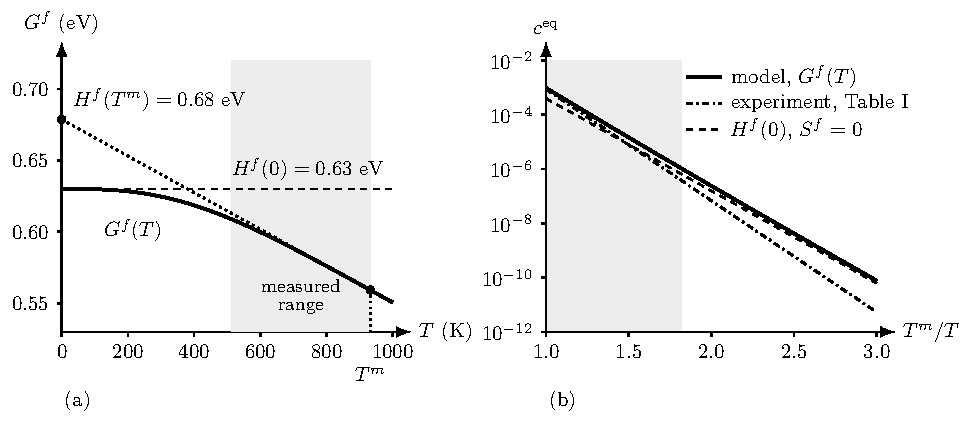
\includegraphics{figures/arrhenius}
\caption{Vacancy formation in Al from a model that reproduces the GGA values of Table~I of [F]. (a) Gibbs energy of formation $G^f(T)$ (solid), the $0$~K enthalpy (dashed) and the tangent at $T^m$ extrapolated to $T = 0$ (dotted). (b) Equilibrium concentration against $T^m/T$ for the model, for the experimental straight line of Table~I and for $H^f(0)$ with $S^f = 0$. Gray: temperatures above $0.55\,T^m$, the range of the experiments.}
\label{fig:arrhenius}
\end{figure}
\begin{parts}
    \item If $H^f$ and $S^f$ do not depend on $T$, what does a plot of $\ln c^{\text{eq}}$ against $1/T$ look like? Which feature of the plot gives $H^f$, and which gives $S^f$? This is Eq.~(42) of [F]. Which line in Fig.~\ref{fig:arrhenius}(b) has this form, and why does the model curve bend toward the dashed line at low temperature?
    \item Evaluate $c^{\text{eq}}(T^m)$ with $g_X = 1$. By what factor would $c^{\text{eq}}$ be smaller if the vibrational formation entropy were zero?
    \item Use $\partial^2G^f/\partial T^2 = -C_P^f/T$, with the formation heat capacity $C_P^f$, as in Section~4 of the note. If $C_P^f > 0$, is $G^f(T)$ concave or convex?
    \item An experiment measures $G^f$ only in the gray range of Fig.~\ref{fig:arrhenius}(a) and extrapolates the tangent line, the dotted line, to $T = 0$. Show that the intercept equals $H^f(T^m)$ and that the slope equals $-S^f(T^m)$. For a concave $G^f(T)$, which is larger, $H^f(T^m)$ or $H^f(0)$? Check the answer against the figure and against Table~I of [F].
    \item In Fig.~\ref{fig:arrhenius}(b), the model and the straight experimental line nearly agree in the gray range but differ by about an order of magnitude at $T^m/T = 3$. What does this difference say about predicting defect concentrations at room temperature from high-temperature data?
\end{parts}
\textit{Answer.} (a) A straight line with the slope $-H^f/k_B$ and the intercept $\ln g_X + S^f/k_B$, the dash-dotted line. The model entropy falls to zero as $T \to 0$, so the model approaches the line with $H^f(0)$ and $S^f = 0$. (b) $H^f/k_BT^m = 9.45$ and $c^{\text{eq}} = 8.7\times10^{-4}$. Without $S^f$, it would be $e^{2.4} = 11$ times smaller. (c) Concave. (d) The tangent of a concave function lies above it, so $H^f(T^m) \ge H^f(0)$. Table~I gives $0.68 > 0.63$~eV (GGA) and $0.78 > 0.68$~eV (LDA), both with anharmonicity. (e) An Arrhenius line fixed in the measured range does not predict the low-temperature concentration, because $S^f$ and $H^f$ change with $T$. The $0$~K values with the temperature dependence of $G^f$ are needed.\\
\textit{Related:} Sections~3.3, 4.5 and~5.3 of the note. \textit{Source:} [F], Secs.~II.B.3 and~II.C.1, Eq.~(42), Table~I.

\paragraph{Exercise 5: Electronic entropy and the Fermi--Dirac distribution.}
Electrons are fermions, so each single-particle orbital holds either $0$ or $1$ electron of a given spin. Non-interacting orbitals are independent.
\begin{parts}
    \item Treat one orbital of energy $\epsilon_i$ as a grand canonical system with $N_i \in \{0, 1\}$, in contact with an electron reservoir at $\mu = E_F$. What is $\Xi_i$? Show that the mean occupation is the Fermi--Dirac function $f_i = 1/[e^{\beta(\epsilon_i - E_F)} + 1]$.
    \item What is the Gibbs--Shannon entropy of a two-outcome distribution with the probabilities $f_i$ and $1 - f_i$? Why does the total entropy add over orbitals? Derive Eq.~(11) of [F]:
    \begin{equation*}
        S^{\text{el}} = -k_B\sum_i\left[(1 - f_i)\ln(1 - f_i) + f_i\ln f_i\right].
    \end{equation*}
    \item Compare part~(b) with the ideal mixing entropy of Section~11.7 of the note. What is ``mixed'' here?
    \item Near $E_F$, let the density of states be a constant $D_F$, counting both spins. Turn the sum into an integral with $x = \beta(\epsilon - E_F)$ and use
    \begin{equation*}
        \int_{-\infty}^{\infty}dx\left[-f\ln f - (1 - f)\ln(1 - f)\right] = \frac{\pi^2}{3},\qquad f = \frac{1}{e^x + 1},
    \end{equation*}
    to show that $S^{\text{el}} = (\pi^2/3)k_B^2TD_F$.
    \item The excitation energy is $\Delta E^{\text{el}} = (\pi^2/6)(k_BT)^2D_F$. Show that $\tilde F^{\text{el}} = \Delta E^{\text{el}} - TS^{\text{el}} = -\tfrac12TS^{\text{el}}$, Eq.~(13) of [F]. Why is this contribution small in a semiconductor but not in a metal?
    \item A neutral defect has one unpaired electron in a localized gap orbital that holds either spin. Which part of $S^{\text{el}}$ survives as $T \to 0$, and where does it reappear in Exercise~3?
\end{parts}
\textit{Answer.} (a) $\Xi_i = 1 + e^{-\beta(\epsilon_i - E_F)}$ and $f_i = -\partial\ln\Xi_i/\partial(\beta\epsilon_i)$. (b) $-k_B[f\ln f + (1 - f)\ln(1 - f)]$, and independent systems have additive entropies (Section~3.2 of the note). (c) Occupied and empty orbitals are ``mixed''. (d) The integral is $\pi^2/3 = 3.290$. (e) $D_F \approx 0$ in the band gap of a semiconductor. (f) $k_B\ln 2$, which is the spin degeneracy $g_X = 2$ in $S^{\text{conf}}$.\\
\textit{Related:} Sections~1.1, 3.2, 5 and~11.7 of the note. \textit{Source:} [F], Sec.~II.A.2, Eqs.~(10)--(13).

\paragraph{Exercise 6: Vibrational free energy and the Bose--Einstein distribution.}
Near equilibrium, the energy of the ions is quadratic in the displacements $u_k = R_k - R_k^0$, Eq.~(9) of [F].
\begin{parts}
    \item Newton's equations read $M_k\ddot u_k = -\sum_l \Phi_{kl}u_l$, with the force constants $\Phi_{kl} = \partial^2F^{\text{el}}/\partial R_k\partial R_l$. Substitute $u_k = w_ke^{-i\omega t}/\sqrt{M_k}$. Why does the dynamical matrix $D_{kl} = \Phi_{kl}/\sqrt{M_kM_l}$, Eq.~(14) of [F], appear, and why are its eigenvalues $\omega_i^2$?
    \item A quantum oscillator has the levels $(n + \tfrac12)\hbar\omega$, $n = 0, 1, 2, \dots$. Sum the geometric series for $Z$. Show that $F = \hbar\omega/2 + k_BT\ln(1 - e^{-\beta\hbar\omega})$, one term of Eq.~(17) of [F].
    \item Show that the mean energy is $(\tfrac12 + \bar n)\hbar\omega$ with $\bar n = 1/(e^{\beta\hbar\omega} - 1)$, Eq.~(16) of [F]. Read $\bar n$ as the mean number of phonons in the mode. Compare $\bar n$ with $f$ of Exercise~5. Which sign changed, and why is the phonon chemical potential zero?
    \item Find the high-temperature limit of $F$. Show that the vibrational formation entropy becomes $S^f_{\text{vib}} = k_B\sum_i\ln(\omega_i^{\text{bulk}}/\omega_i^{\text{def}})$, with equal numbers of modes on both sides.
    \item Around a vacancy, the bonds of the neighbor atoms are broken. Do their modes soften or stiffen, and what is the sign of $S^f_{\text{vib}}$? Estimate $S^f_{\text{vib}}$ if the $36$ modes of the $12$ nearest neighbors in an fcc metal soften by $5\%$, and compare with $S^f = 2.4\,k_B$ for Al.
\end{parts}
\textit{Answer.} (a) The substitution turns the equations into the eigenvalue problem $Dw = \omega^2w$, Eq.~(15) of [F]. $D$ is real and symmetric, and stability makes it positive definite. (b) $Z = e^{-\beta\hbar\omega/2}/(1 - e^{-\beta\hbar\omega})$. (c) $-1$ replaces $+1$ in the denominator, because any number of phonons can occupy a mode. Phonon numbers are not conserved. (d) $F \to k_BT\ln(\hbar\omega/k_BT)$. (e) The modes soften, and $S^f_{\text{vib}} > 0$. The estimate gives $36\ln(1/0.95) = 1.8\,k_B$.\\
\textit{Related:} Sections~3, 3.3 and~4.5 of the note. \textit{Source:} [F], Sec.~II.A.3, Eqs.~(9), (14)--(17).

\paragraph{Exercise 7: Formation volume and pressure.}
At finite $T$ and $P$, the formation Gibbs energy of Eq.~(23) of [F] contains the term $PV^f$, with the formation volume $V^f = \Omega' - \Omega$.
\begin{parts}
    \item Which derivative of $G^f(T, P)$ gives $V^f$? Use Section~5.3 of the note.
    \item Show that $(\partial\ln c^{\text{eq}}/\partial P)_T = -V^f/k_BT$. For a vacancy in Al with $V^f = 11$~\AA$^3$, by what factor does $1$~GPa change $c^{\text{eq}}$ at $900$~K?
    \item A supercell of fixed volume $V_0$ prevents the relaxation $V^f$. Use $B = -V\,\partial P/\partial V$ to show that the elastic energy stored is $\Delta E \approx B(V^f)^2/(2V_0)$, Eq.~(57) of [F]. Evaluate $\Delta E$ for $B = 100$~GPa, $V^f = 10$~\AA$^3$ and $V_0 = 1000$~\AA$^3$.
    \item How does $\Delta E$ scale with the supercell size $L$? Why does stability, $B > 0$, make the constant-volume energy higher than the relaxed energy?
\end{parts}
\textit{Answer.} (a) $V^f = (\partial G^f/\partial P)_T$. (b) $\Delta\ln c = -0.89$, so $c$ drops by a factor of $2.4$. (c) $\Delta E = \int_0^{V^f}B\,(V/V_0)\,dV = 31$~meV. (d) $\Delta E \propto 1/L^3$. The constrained state lies on a convex $F(V)$ away from the minimum.\\
\textit{Related:} Sections~4.1, 4.6 and~5.3 of the note. \textit{Source:} [F], Secs.~II.B.1 and~III.D, Eqs.~(23), (57).

\paragraph{Exercise 8: Chemical potentials and the stability window.}
A nitrogen vacancy $V_{\text{N}}$ forms in GaN, which coexists either with Ga metal or with N$_2$ gas.
\begin{parts}
    \item In GaN at equilibrium, why must $\mu_{\text{Ga}} + \mu_{\text{N}} = \mu(\text{GaN})$, Eq.~(26) of [F]? Use the Euler relation $G = \sum_i\mu_iN_i$ of Section~5.5 of the note.
    \item If $\mu_{\text{Ga}}$ exceeded $\mu_{\text{Ga}}(\text{Ga metal})$, what would form? Derive the bounds of Eqs.~(27)--(30) of [F] and show that
    \begin{equation*}
        \Delta_fG^0(\text{GaN}) \le \Delta\mu_{\text{Ga}} \le 0,\qquad \Delta\mu_{\text{N}} = \Delta_fG^0(\text{GaN}) - \Delta\mu_{\text{Ga}},
    \end{equation*}
    in the notation of Eqs.~(31)--(34).
    \item Draw $g(X)$ for the Ga--N system at fixed $(T, P)$, with three line phases at $X = 0$ (Ga), $X = 1/2$ (GaN) and $X = 1$ (N$_2$), and construct the convex hull of Section~11.4 of the note. Which tangent lines touch the GaN point? Show that their intercepts at $X = 0$ and $X = 1$ sweep exactly the window of part~(b).
    \item The formation of $V_{\text{N}}$ removes one N atom, $n_{\text{N}} = -1$. How much larger is $E^f(V_{\text{N}})$ under N-rich than under Ga-rich conditions?
    \item For N$_2$ gas, the molecule has the ground energy $E(\text{N}_2)$ and the rotational partition function $z_{\text{rot}} = k_BT/(\sigma B_0)$ for $k_BT \gg B_0$. Start from $\mu = k_BT\ln(P\lambda_{\text{th}}^3/k_BT)$ of Exercise~13 of \texttt{exercise.pdf} and multiply $Z_N$ by $z_{\text{int}}^N$. Derive Eq.~(35) of [F]:
    \begin{equation*}
        2\mu_{\text{N}} = E(\text{N}_2) + k_BT\ln\frac{PV_Q}{k_BT} + k_BT\ln\frac{\sigma B_0}{k_BT} + \mu_{\text{vib}},\qquad V_Q = \lambda_{\text{th}}^3.
    \end{equation*}
    \item Raising $P(\text{N}_2)$ at fixed $T$ moves $\mu_{\text{N}}$ in which direction? How does $c(V_{\text{N}})$ respond?
\end{parts}
\textit{Answer.} (b) Excess Ga would precipitate as metal, and excess N would leave as N$_2$. (c) The tangents through the GaN point rotate between the slopes of the Ga--GaN and GaN--N$_2$ segments of the hull. (d) By $|\Delta_fG^0(\text{GaN})|$, about $1$~eV. (e) $\mu = -k_BT\ln z_{\text{int}} + k_BT\ln(P\lambda_{\text{th}}^3/k_BT)$, with $z_{\text{int}} = e^{-\beta E(\text{N}_2)}z_{\text{rot}}z_{\text{vib}}$. (f) $\mu_{\text{N}}$ rises by $\tfrac12k_BT\,\Delta\ln P$, and $c(V_{\text{N}}) \propto P^{-1/2}$.\\
\textit{Related:} Sections~5.5, 5.7, 11.3 and~11.4 of the note. \textit{Source:} [F], Sec.~II.B.2, Eqs.~(26)--(35).

\paragraph{Exercise 9: Charge neutrality and the Fermi level.}
A semiconductor has the band gap $E_g$, parabolic bands with the effective masses $m_e$ and $m_h$, and dilute charged defects. Electrons and holes follow Exercise~5.
\begin{parts}
    \item Why must the crystal as a whole be neutral, Eq.~(36) of [F]? Which unknown does this condition fix, once all $c(X^q)$ are written as functions of $E_F$?
    \item The conduction band has the density of states per volume
    \begin{equation*}
        D_c(E) = \frac{1}{2\pi^2}\left(\frac{2m_e}{\hbar^2}\right)^{3/2}\sqrt{E - E_c},
    \end{equation*}
    with both spins included. When $E_c - E_F \gg k_BT$, which term of the Fermi--Dirac denominator can be dropped? Show that $n_e = N_ce^{-(E_c - E_F)/k_BT}$ with $N_c = 2(m_ek_BT/2\pi\hbar^2)^{3/2}$. Compare with Eq.~(38) of [F], which counts one spin.
    \item Evaluate $N_c$ for $m_e$ equal to the free-electron mass at $300$~K.
    \item Without defects, $n_e = n_h$. Show that $E_F = E_g/2 + \tfrac34k_BT\ln(m_h/m_e)$.
    \item A donor $D^+$ has $E^f = E_D + E_F$, and a native acceptor $A^-$ has $E^f = E_A - E_F$, with $c \propto e^{-E^f/k_BT}$. If the defects outnumber the free carriers, where does neutrality pin $E_F$? Locate this point in a plot of $E^f$ against $E_F$.
    \item Raising the dopant chemical potential $\mu_D$ lowers $E_D$ by the same amount. Show that $E_F$ then rises only by half of the increase of $\mu_D$. Why does this effect, self-compensation, limit doping (Sec.~I.A.2 of [F])?
\end{parts}
\textit{Answer.} (a) The crystal has no external source of charge, so neutrality fixes $E_F$. (b) $f \approx e^{-\beta(E - E_F)}$, and the integral is a Gaussian integral. (c) $N_c = 2.5\times10^{19}$~cm$^{-3}$. (d) $N_c/N_v = (m_e/m_h)^{3/2}$. (e) $c(D^+) = c(A^-)$ gives $E_F = (E_A - E_D)/2$, where the two lines cross. (f) $E_F = (E_A - E_D)/2$ rises by $\Delta\mu_D/2$. Each added donor is compensated by a new acceptor, so the carrier density barely grows.\\
\textit{Related:} Sections~5, 5.5 and~10.3 of the note. \textit{Source:} [F], Secs.~I.A.2 and~II.B.2c, Eqs.~(36)--(38).

\paragraph{Exercise 10: Vacancies close to the melting point.}
Section~V.B of [F] asks whether vacancies cause the rise of the heat capacity of Al close to $T^m$.
\begin{parts}
    \item From Eq.~(40) of [F], the vacancy contribution to the Gibbs energy per site is $\Delta G = -k_BTc^{\text{eq}}(T)$. Use $H = -T^2\,\partial(G/T)/\partial T$ to show that $\Delta H = c^{\text{eq}}H^f$. Why is this result expected?
    \item Show that $\Delta C_P = k_Bc^{\text{eq}}(H^f/k_BT)^2$.
    \item The number of vacancies in $N$ sites is a sum of nearly independent site occupations. What is its variance? Use $\mathrm{Var}(U) = k_BT^2C$ of Section~3.3 of the note to obtain part~(b) a second way.
    \item Evaluate $\Delta C_P$ per atom for Al at $T^m$ with the data of Exercise~4, and compare it with $3k_B$.
    \item Which other response function of Section~V.B of [F] should reveal vacancies, and why does it depend on $V^f$?
\end{parts}
\textit{Answer.} (a) Each vacancy carries the enthalpy $H^f$. (c) $\mathrm{Var}(n) \approx n$, so $\mathrm{Var}(U) = (H^f)^2n$. (d) $\Delta C_P = 0.078\,k_B$ per atom, about $2.6\%$ of $3k_B$. (e) The thermal expansion coefficient, because each vacancy adds $V^f$ to the volume.\\
\textit{Related:} Sections~3.3, 4.6 and~5.3 of the note. \textit{Source:} [F], Secs.~II.B.3 and~V.B, Eq.~(40).

\paragraph{Exercise 11: Optical levels and the configuration-coordinate diagram.}
In Fig.~8 of [F], the substitutional acceptor $\text{N}_{\text{O}}$ in ZnO has the absorption energy $E_{\text{abs}} = 2.4$~eV and the emission energy $E_e = 1.7$~eV. ZnO has $E_g = 3.4$~eV.
\begin{parts}
    \item Model the two states $\text{N}_{\text{O}}^-$ and $\text{N}_{\text{O}}^0 + e^-_{\text{CB}}$ by parabolas $\tfrac12K(Q - Q_-)^2$ and $E_{\text{ZPL}} + \tfrac12K(Q - Q_0)^2$ with equal curvature $K$. Why do absorption and emission occur at fixed $Q$ (Franck--Condon principle)?
    \item Show that $E_{\text{abs}} = E_{\text{ZPL}} + E_{\text{rel}}$ and $E_e = E_{\text{ZPL}} - E_{\text{rel}}$, with $E_{\text{rel}} = \tfrac12K(Q_- - Q_0)^2$. Find $E_{\text{rel}}$, the Stokes shift and $E_{\text{ZPL}}$.
    \item The zero-phonon line equals $E_g - \varepsilon(0/-)$. Find $\varepsilon(0/-)$ and compare with $1.3$~eV in [F].
    \item Why does a Fermi-level-dependent concentration use the thermodynamic level, whereas an absorption spectrum uses the optical level? Compare the time scales of electronic and ionic motion.
    \item For a typical phonon energy $\hbar\omega = 40$~meV, how many phonons does the relaxation emit? Why does this number broaden the emission band?
\end{parts}
\textit{Answer.} (b) $E_{\text{rel}} = 0.35$~eV, the Stokes shift is $0.7$~eV, and $E_{\text{ZPL}} = 2.05$~eV. (c) $\varepsilon(0/-) = 1.35$~eV. (d) Electronic transitions take about $10^{-15}$~s, ionic relaxation about $10^{-13}$~s. (e) About $E_{\text{rel}}/\hbar\omega \approx 9$ phonons.\\
\textit{Related:} Sections~3 and~10 of the note. \textit{Source:} [F], Sec.~II.E, Fig.~8, Eq.~(43).

\paragraph{Exercise 12: Diffusion by vacancy hopping.}
Section~I.A.3 of [F] states that impurities usually diffuse with the help of vacancies or interstitials. This exercise builds the diffusion coefficient from the canonical ensemble.
\begin{parts}
    \item An atom makes uncorrelated jumps of length $a$ in random directions, $\Gamma$ jumps per unit time. Why do the cross terms $\langle\vec a_j\cdot\vec a_k\rangle$, $j \neq k$, vanish? Show that $\langle r^2\rangle = \Gamma a^2t$, and define $D$ by $\langle r^2\rangle = 6Dt$.
    \item Check that $c(\vec r, t) \propto t^{-3/2}e^{-r^2/4Dt}$ solves $\partial c/\partial t = D\nabla^2c$ and has $\langle r^2\rangle = 6Dt$.
    \item In one dimension, an atom sits in a well of curvature $K$ and mass $m$, so that the attempt frequency is $\nu = \sqrt{K/m}/2\pi$, and a barrier of height $E_m$ separates the well from the next one. In canonical equilibrium, what is the probability density of finding the atom at the barrier top, normalized over the well? What is the mean forward velocity $\langle v\,\theta(v)\rangle$ from the Maxwell distribution? Multiply the two to show that the jump rate is $\Gamma_0 = \nu e^{-E_m/k_BT}$, the result of transition-state theory.
    \item An atom in a crystal jumps only into a neighboring vacancy. With $z$ neighbors and the vacancy concentration $c_v^{\text{eq}}$ of Exercise~3, show that the self-diffusion coefficient is
    \begin{equation*}
        D = \frac{f_c\,z\,a^2\nu}{6}\exp\!\left(\frac{S^f}{k_B}\right)\exp\!\left(-\frac{H^f + E_m}{k_BT}\right),
    \end{equation*}
    where the correlation factor $f_c$ ($0.78$ for fcc) corrects for jumps straight back into the same vacancy.
    \item Which energy does an Arrhenius plot of $D$ measure? For Al, with $H^f = 0.67$~eV and $E_m = 0.61$~eV, compare with the measured activation energy of about $1.3$~eV.
    \item Section~I.A.3 of [F] says that interstitials move more readily than vacancies but are less abundant. Which sum decides the mechanism that dominates diffusion?
    \item In a non-uniform crystal, the flux is $J = -(Dc/k_BT)\,\partial\mu/\partial x$. For a dilute species with $\mu = k_BT\ln c + \text{const}$, recover Fick's law. Why does this result agree with the statement of Section~11.11 of the note that no flux flows through a two-phase zone?
\end{parts}
\textit{Answer.} (a) Independent jumps have zero mean. (c) The density at the barrier top, normalized over the well, is $\sqrt{K/2\pi k_BT}\,e^{-\beta E_m}$, and $\langle v\,\theta(v)\rangle = \sqrt{k_BT/2\pi m}$. (e) $H^f + E_m = 1.28$~eV. (f) $H^f + E_m$ for each mechanism. (g) $J = -D\,\partial c/\partial x$. Inside a two-phase zone $\mu$ is uniform, so $J = 0$.\\
\textit{Related:} Sections~3, 11.4 and~11.11 of the note. \textit{Source:} [F], Secs.~I.A.3 and~II.B.3, Eq.~(41).

\paragraph{Exercise 13: Charged defects in a periodic supercell.}
A supercell calculation repeats one charged defect $q$ on a cubic lattice of period $L$ in a medium of dielectric constant $\varepsilon$.
\begin{parts}
    \item Why does the electrostatic energy of a periodic array of net charges diverge? Why does a uniform compensating background remove the divergence? What happens to the $\vec G = 0$ Fourier component of the potential?
    \item On dimensional grounds, how must the spurious interaction scale with $q$, $\varepsilon$ and $L$? For a simple cubic array of point charges in a background, the Madelung energy is $E_M = \alpha_Mq^2/(2\varepsilon L)$ with $\alpha_M = 2.8373$. Evaluate $E_M$ for $q = 1$, $\varepsilon = 10$ and $L = 12$~\AA.
    \item The computational cost grows as the cube of the number of atoms. By what factor does the cost grow if the error is halved? This is the estimate of Sec.~I.C.2 of [F].
    \item The energy behaves as $E(L) = E_\infty + a_1/L + a_3/L^3$, with an $L^{-3}$ term from the quadrupole moment. How many supercell sizes determine $E_\infty$? How many if $a_1$ is taken from the Madelung energy?
    \item Why is the Fermi level of Exercise~1 undefined in a charged supercell until the average electrostatic potential is aligned with that of the bulk (Fig.~12 of [F])?
\end{parts}
\textit{Answer.} (a) The Coulomb sum over the net charges grows with the number of cells. The background sets the average charge, the $\vec G = 0$ term, to zero. (b) $E_M \propto q^2/(\varepsilon L)$, and $E_M = 0.17$~eV, larger than many target accuracies. (c) Halving the error doubles $L$, so the number of atoms grows $8$ times and the cost $8^3 = 512$ times. (d) Three sizes, or two with $a_1$ known. (e) $E^f$ contains $qE_F$, and $E_F$ is measured from the VBM, whose absolute energy depends on the reference of the potential.\\
\textit{Related:} Section~5.2 of the note. \textit{Source:} [F], Secs.~I.C.2 and~III.C.

\end{document}
